% TODO?: fazer uma tabela comparativa entre os artigos

\section{Fundamentação Teórica}

\subsection {LSTM}

\acrfull{LSTM} é amplamente utilizado para predição de tráfego e de informações que derivam de dados sequenciais/séries temporais, sendo possível encontrar diversos trabalhos na literatura que mostram sua eficiência quando comparado a outros métodos. Como descrito em \cite{Zainab_2018} e em \cite{Xiaolei_2015}, \acrshort{LSTM} é um tipo de \acrfull{RNN} que utiliza de estados anteriores e do estado atual da rede para gerar sua saída. Ao utilizar dos estados anteriores, a \acrshort{RNN} acaba por simular uma memória, melhorando seu aprendizado. 

\begin{figure}[htb]
    \centering
    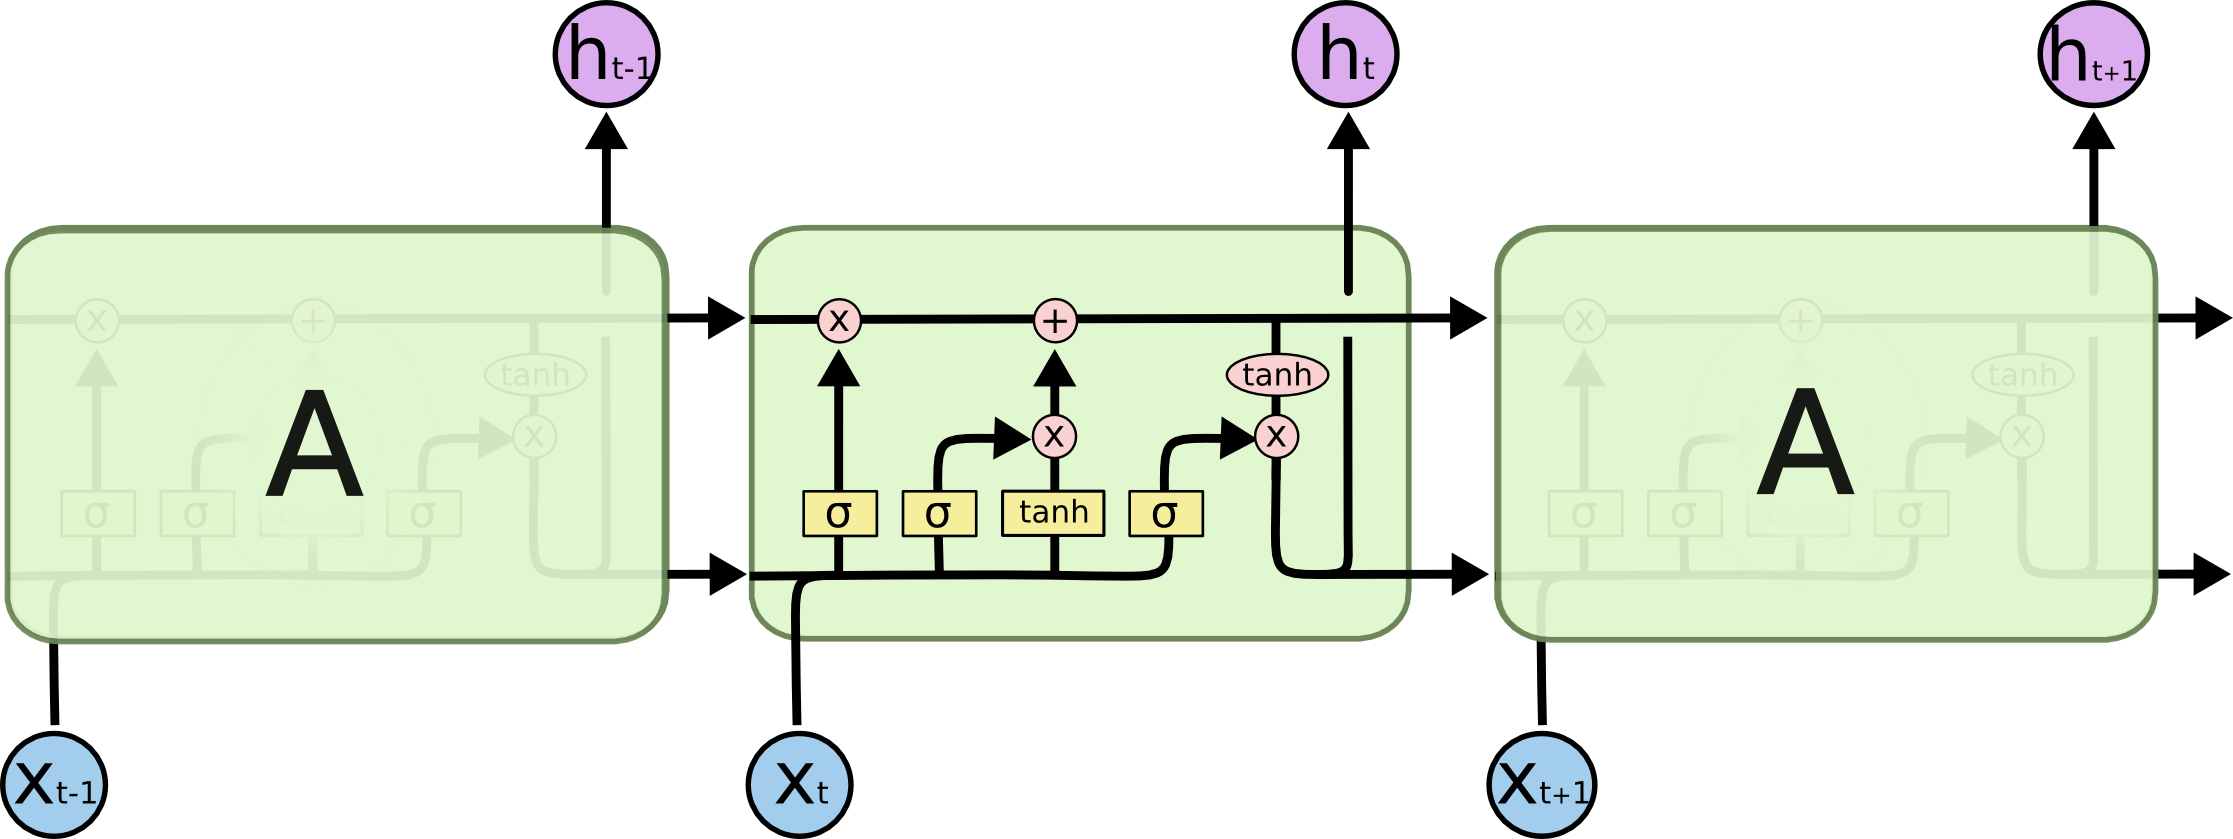
\includegraphics[scale=0.4]{lstm3.png}
    \label{figure:eixo}
    \caption[Representação de uma arquitetura LSTM]{Representação de uma arquitetura LSTM\footnotemark}
\end{figure}

\footnotetext{https://colah.github.io/posts/2015-08-Understanding-LSTMs/}

Porém, diferentemente de uma \acrshort{RNN}, o LSTM possui uma unidade a mais em seus blocos chamada de célula de memória. Esta célula é capaz de perceber as características mais latentes dos dados e descartar as menos importantes. Assim, o \acrshort{LSTM} consegue manter as características mais importantes na rede por mais tempo que uma \acrfull{RNN} comum. Por estes motivos, o \acrshort{LSTM} é excelente para modelar séries temporais e dados sequenciais.

\subsection {GAN}

Introduzida em 2014 pelo trabalho\cite{NIPS2014_5423}, esta arquitetura utiliza de dois modelos, um gerador e um discriminador, que competem entre si. O objetivo do gerador é produzir em sua saída informações similares às contidas nos dados de entrada. Já o objetivo do discriminador é distinguir os dados produzidos pelo gerador dos dados originais. Ou seja, o objetivo principal da \acrshort{GAN} é treinar um gerador, assim fazendo com que o discriminador não consiga mais diferenciar os dados originais dos dados gerados. Até por isso, os discriminadores são normalmente descartados no final de um treinamento \cite{turner2018metropolis}.

\begin{figure}[htb]
    \centering
    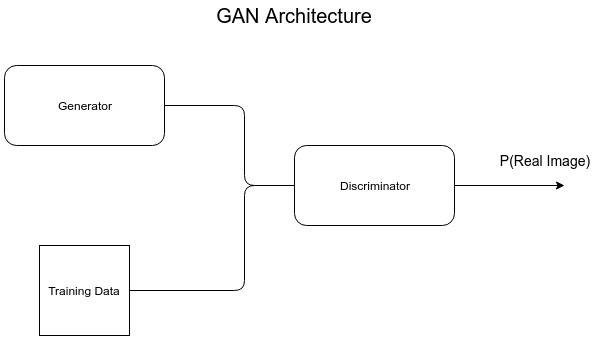
\includegraphics[scale=0.5]{gan.png}
    \label{figure:eixo}
    \caption[Representação de uma arquitetura GAN]{Representação de uma arquitetura GAN\footnotemark}
\end{figure}

\footnotetext{https://www.oreilly.com/library/view/deep-learning-quick/9781788837996/029fffd7-ce97-40de-993e-5f47dcc01c15.xhtml}

%Para fazer a previsão será utilizada \acrfull{GAN}. \acrshort{GAN} é um método que utiliza dois modelos para serem o gerador e o discriminador. O trabalho do gerador é tentar reproduzir algo. O trabalho do discriminador é avaliar o que o gerador fez e decidir se é bom o suficiente. \acrshort{GAN} põe dois modelos para treinarem juntos como rivais. Neste trabalho escolhemos como modelo gerador a \acrshort{LSTM} e como modelo discriminador o --indefinido--


% Falar sobre GAN
% e é possível encontrar pesquisas na área de geração de imagens a partir de textos \cite{reed2016generative}.

% Falar sobre o problema da GAN para os nossos dados
%Porém essas pesquisas utilizam de dados independentes e a \acrshort{GAN} tentava descobrir a distribuição desses dados. No caso deste trabalho, os dados estão associados a um tempo, o que dá a eles uma certa dependência entre si (esses dados ocorrem antes desses outros). Mas mesmo assim, existem trabalhos que também utilizam \textit{time series} e 
%Nesses trabalhos são usados variações da \acrshort{GAN} para que ela seja capaz de trabalhar com \textit{time series}. Sendo uma das variações a \acrfull{InfoGAN} \cite{chen2016infogan}, \acrfull{ACGAN} \cite{odena2017conditional} e \acrfull{RCGAN} \cite{esteban2017real}.

% Falar da otimização (MH-GAN)
%Além disso, é possível melhorar a performance do gerador de uma \acrshort{GAN} utilizando o discriminador que normalmente é jogado fora, segundo . \acrfull{MH-GAN} teve resultados promissores.

\section{Trabalhos Relacionados}

Em \cite{Zainab_2018}, é apresentado um trabalho de predição de tráfego que tem como objetivo prever congestionamentos em vias de Estocolmo, Suécia, utilizando aprendizagem profunda \acrfull{SLSTM}. Para tal, são utilizados dados coletados por sensores do \textit{motorway control system} da cidade. Tais sensores monitoram as principais vias da metrópole e coletam informações como fluxo e velocidade de cada faixa a cada 1 minuto. Neste contexto, o autor sugere uma metodologia em que as vias são particionadas em seções e, sobre cada seção, é aplicado o \acrshort{LSTM}, pois considerar a via como um todo poderia ser muito custoso computacionalmente devido a quantidade total de sensores. O trabalho propõe três modelos de predição:

\begin{itemize}
    \item O (1-1) Modelo utilizando apenas um sensor que faz a predição apenas do local daquele sensor
    \item O (n-n) Modelo que utiliza n sensores de uma determinada área e faz a predição de todas as localidades
    \item O (m-n) Modelo que utiliza os m sensores mais significantes de uma área que contém um total de n sensores e que faz a predição para todos os n locais.
\end{itemize}

Dos três modelos apresentados, o mais eficiente foi o m-n, pois faz a previsão de tráfego em vários pontos diferentes da via e tem um custo computacional menor que o n-n, além disso utiliza menos sensores, o que diminui os dados de entrada da rede neural. Para validar os resultados das predições, a acurácia dos resultados é calculada utilizando \acrshort{RMSE} e \acrshort{MAE}. O resultado dessas métricas é comparado com a acurácia de outros modelos de predição, como \acrfull{RNN} e \acrfull{FFN}. O erro foi menor na metodologia do autor em todos os casos, comprovando a eficácia do método. 

Já em \cite{lv_6894591}, um trabalho semelhante de comparação de modelos de predição, mas utilizando \acrfull{SAE}. O modelo de predição proposto pelo artigo é aplicado aos dados coletados por 15000 sensores espalhados pelas estradas da Califórnia. As predições são divididas em intervalos de 15, 30, 45 e 60 minutos. Mais uma vez, a acurácia das predições foi medida utilizando  \acrshort{MAE}, \acrshort{MRE} e \acrshort{RMSE} para cada intervalo de tempo e comparada a acurácia de predição de outros métodos, como \acrfull{BPNN}, \acrfull{RW}, \acrfull{SVM} e \acrfull{RBFNN}. Mais uma vez, o método apresentado pelo artigo foi mais eficiente que os outros a qual ele foi comparado.      

Em \cite{NIPS2014_5423} é apresentado a \acrfull{GAN} para criar um framework de estimativa. São utilizados dois modelos sendo um o gerador e outro o discriminador. O modelo gerador é alimentado com diversas imagens de um banco de imagens e tem como papel recriar essas imagens o mais fielmente possível, enquanto o modelo discriminador tenta separar quais imagens foram criadas pelo gerador e quais vieram do banco. Dessa forma, os modelos competem entre si, melhorando suas estimativas em cada iteração, até que não seja mais possível diferenciar as imagens geradas pelo modelo gerador das imagens do banco.

Em \cite{banushev_2019} utiliza da \acrshort{GAN} para prever as flutuações de um mercado de ações, mais especificamente os dados coletados das flutuações das ações da empresa Goldman Sachs dentre o período de 1 de Janeiro de 2010 até 31 de Dezembro de 2018. 80 por cento dos dados foram utilizados para treinamento e 20 por cento para testes (Os últimos 800 dias). Neste contexto, O LSTM foi utilizado como gerador e uma CNN foi utilizada como discriminadora. Após alimentar os algoritmos com os dados, o trabalho comparou estas previsões dos últimos 800 dias com os valores reais coletados das flutuações da Goldman Sachs e tiveram resultados promissores.

%\subsection{RNN}

%Redes neurais recorrentes são um tipo de rede neural aonde a saída depende não somente da entrada, mas também dos estados anteriores da rede, o que acaba por agir como um tipo de memória. Neste trabalho, utilizamos uma variação desse tipo de rede neural chamada \acrfull{LSTM}.


%\subsection{LSTM}

%O LSTM é primeiramente citado em \cite{Felix_1999} aonde o autor define pela primeira vez o seu conceito e funcionamento. Com o passar dos anos e o aumento do número dos carros nas rodovias, o LSTM foi rapidamente inserido no contexo de traffic prediction flow. Existem diversos artigos e trabalhos a respeito do seu uso dentro deste assunto. Um dos mais relevantes deles é o \cite{Xiaolei_2015}, aonde o autor faz uma comparação do desempenho do LSTM com outros métodos de predição. 

%    - Entrada: Camada que recebe os dados 
%    - \arcshort{LSTM}: (camada aonde ocorre a recursão dos dados e as células de memória são atualizadas, %decidindo o que continua na rede e o que é esquecido)
%    - Saída:  

%\subsection{GAN}



%\subsection{MH-GAN}

%No caso, o artigo de previsão de ações utilizou uma variação da \acrshort{GAN} desenvolvida pela \textit{Uber} e tiveram resultados que superaram o estado da arte. A empresa estadunidense introduziu a \acrfull{MH-GAN} em \cite{turner2018metropolis} que tem como objetivo fazer com que a \acrshort{GAN} sirva para treinar o gerador. 